\graphicspath{{C:/Users/Maxime Muller/Documents/Latex/Phytheme/Complement-cinematique/Figures}}
\chapter{Mouvement dans un champ de force centrale newtonien}
\section{Force centrale conservative}
\subsection{Force centrale}
\begin{definition}[force centrale]
    On considère un point \(M\) de masse \(m\) soumis à une force \(\vv{F}\). \(\vv{F}\) est une force centrale si on a : 
    \[
        \vv{F} = F \cdot \vv{u}_{r}
    \]  
    ie la norme de la force ne dépend que de la distance à un point \(O\) origine.
\end{definition}

\begin{figure}[!htb]
    \centering
    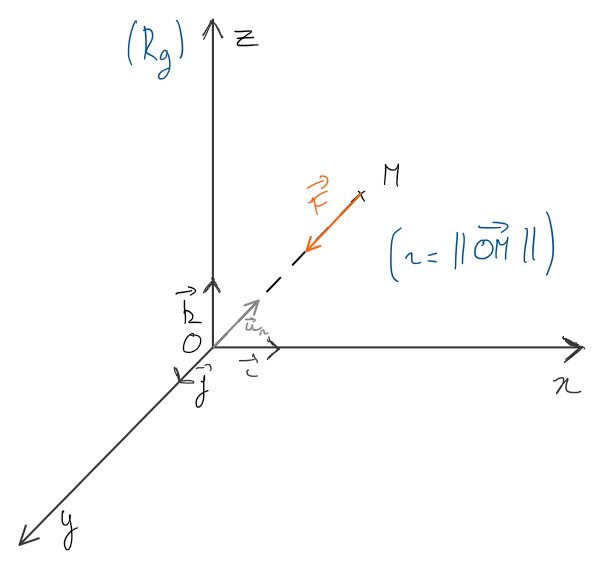
\includegraphics[width=0.4 \textwidth]{SCHEMA3-1.png}
    \caption{Schema d'une force centrale}
    \label{fig:SCHEMA3-1}
\end{figure}

\begin{eg}[Exemple]
    Cette force est dirigée vers le point \(O\), le centre de force. Le point \(O\) est immobile dans le réferentiel \((Rg)\). 
\end{eg}



\subsection{Force conservative}
\begin{definition}[Force conservative]
    Une force conservative est une force qui dérive d'une énergie potentielle.
    \[
        \vv{F} = -\grad E_{p}
    \]
\end{definition}

\begin{corollary}[En coordonnées sphériques]
    En coordonnées sphériques on a : 
    \[
        d \vv{OM} = dr\vv{u}_{r} + r d \theta\vv{u}_{\theta} + r \sin \theta d \phi \vv{u}_{\phi}
    \]
    \[
        \implies \grad E = \frac{\partial E}{\partial r} \vv{u}_{r} + \frac{1}{r}\frac{\partial E}{\partial \theta} + \vv{u}_{\theta} + \frac{1}{r\sin \theta}\frac{\partial E}{\partial \phi} \vv{u}_{\phi} 
    \]
\end{corollary}

\begin{corollary}[Dans le cas d'une force centrale]
    Dans le cas d'une force centrale, l'énergie potentielle ne dépend que de \(r = \lVert \vv{OM} \rVert \). On a alors : 
    \[
        \vv{F}(r) = - \frac{dE_{p}(r)}{dr} \vv{u}_{r}
    \]
\end{corollary}

\subsection{Champ de force centrale newtonien}

\begin{definition}[Champ de force centrale newtonien]
    Si la force centrale \(\vv{F}\) est telle que \(\lVert \vv{F} \rVert \propto \frac{1}{r^{2}}\), et que le centre de force est fixe dans le réferentiel galliléen d'étude, on parle de champ de force centrale newtonien.  
    \[
        \vv{F}(r) = \frac{k}{r^{2}} \vv{u}_{r}, k = \text{cste }
    \]
\end{definition}

\begin{eg}[Exemple]
    \begin{itemize}
        \item La loi de gravitation de Newton :\(\vv{F} = -\frac{GmM}{r^{2}}\vv{u}_{r}\)
        \item La loi de Coulomb : \(\vv{F}_{e} = \frac{1}{4\pi \epsilon_{0}} \frac{qq'}{r^{2}} \vv{u}_{r} \)  
    \end{itemize}
\end{eg}


\section{Lois de conservation}
\subsection{Conservation du moment cinétique : loi des aires}

D'après le \autoref{col:TMC}, on a :
\[
    \boxed{\frac{d}{dt}\vv{L}_{0} = \vv{OM} \wedge \vv{F}}
\]

Or pour une force centrale, \(\vv{F} = F(r) \vv{u}_{r}\), d'où : 
\[
    \frac{d}{dt}\vv{L}_{0} = \vv{OM} \wedge F(r) \cdot \vv{u}_{r} = 0 
\] 

D'où, pour un champ de force centrale, le moment cinétique est constant. \par

\begin{figure}[!htb]
    \centering
    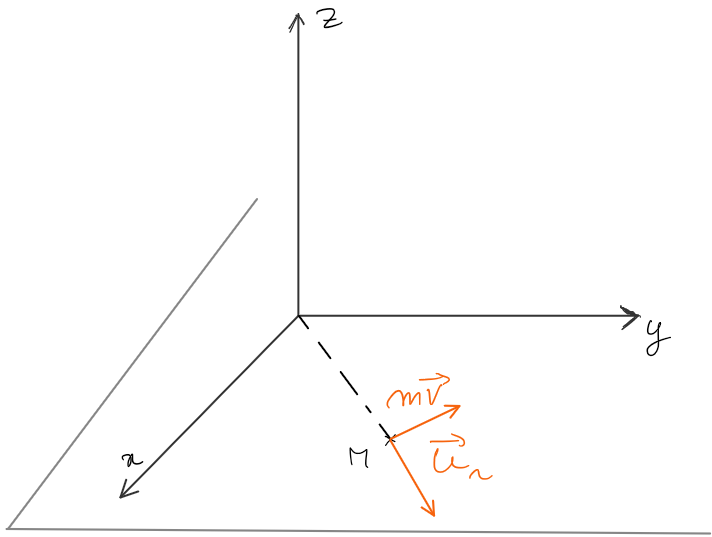
\includegraphics[width=0.4 \textwidth]{SCHEMA3-2.png}
    \caption{Schema de vitesse et position}
    \label{fig:SCHEMA3-2}
\end{figure}



Or : \(\vv{u}_{r} \wedge  \vv{u}_{\theta} = \vv{u}_{z}\), donc le moment cinétique est à tout instant normal au plan \(\vv{OM}; m\vv{v}\). Si on se place en coordonnées cylindro-polaires :
\[
    \begin{cases}
        \vv{OM} = r\vv{u}_{r}\\
        \vv{v} = \dot{r}\vv{u}_{r} + r \dot{\theta} \vv{u}_{\theta}
    \end{cases}
\]
   
\begin{eqnarray*}
    \implies \vv{L}_{0} &=& \vv{OM} \wedge m\vv{v} \\
    &=& r\vv{u}_{r} \wedge m(\dot{r}\vv{u}_{r} + r \dot{\theta} \vv{u}_{\theta}) \\
    &=& r^{2}\dot{\theta} \vv{u}_{r} \wedge  m\vv{u}_{\theta} \\
    &=& mr^{2}\dot{\theta} \vv{u}_{z}\\
    \implies mr^{2}\dot{\theta} &=& \text{cste } \\
    \implies r^{2}\dot{\theta} &=& \text{cste } = l
\end{eqnarray*}

\subsubsection{Inteprétation : Loi des aires}

\begin{figure}[!htb]
    \centering
    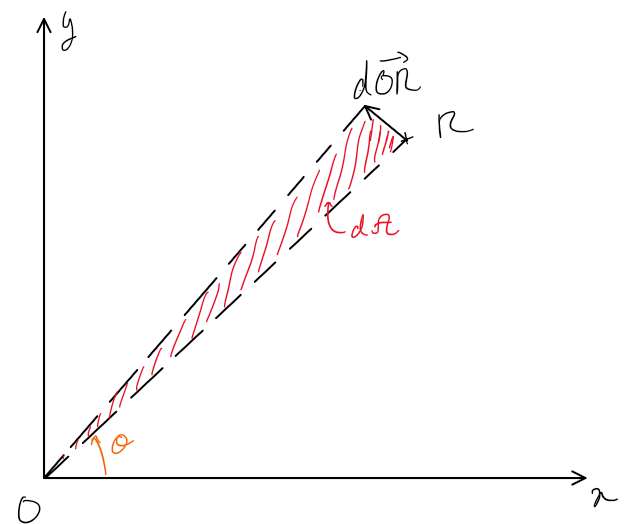
\includegraphics[width=0.4 \textwidth]{SCHEMA3-3.png}
    \caption{Schema de l'aire balayée}
    \label{fig:SCHEMA3-3}
\end{figure}



\[
    d \mathcal{A} = \frac{1}{2}\lVert \vv{OM} \wedge d \vv{OM} \rVert 
\]

Or \(\vv{v} = \frac{d}{dt}\vv{OM} \implies d\vv{OM} = \vv{v}dt\)
\begin{eqnarray*}
    \implies d \mathcal{A} &=& \lVert \vv{OM} \wedge \vv{v}dt \rVert \frac{1}{2} \\
    &=& \frac{1}{2}\lVert r\vv{u}_{r} \wedge (\dot{r}\vv{u}_{r} + r \dot{\theta}\vv{u}_{\theta}) \rVert dt \\
    \implies \frac{d \mathcal{A}}{dt} &=& \frac{1}{2} \lVert \vv{OM} \wedge \vv{v} \rVert \\
    &=& \frac{1}{2}\lVert \vv{L}_{0} \rVert \\
    &=& \frac{l}{2}\\
    \implies && \boxed{\Delta \mathcal{A} = \frac{l}{2}\Delta t} 
\end{eqnarray*}

Ainsi, on a montré que l'aire ballayée est constante pour un temps donné, c'est la deuxième loi de Kepler : la loi des aires.

\subsection{Conservation de l'énergie mécanique}

La force est conservative, on a donc : 
\begin{align*}
    E_{m} &= E_{c} + E_{p}  = \text{cste } \\
    \implies E_{m} &= \frac{1}{2}mv^{2} + E_{p}(r) \\
    \text{ Or } \vv{v} &=  \dot{r}\vv{u}_{r} + r\dot{\theta} \vv{u}_{\theta} \\
    \implies v^{2} &= \vv{v} \cdot \vv{v} = \dot{r}^{2} + r^{2} \dot{\theta}^{2} \\
    \text{ Or } r^{2}\dot{\theta} &= \text{cste } = l \implies \dot{\theta} = \frac{l}{r^{2}} \\
    \implies E_{m} &= \frac{1}{2} (\dot{r}^{2} + \frac{c^{2}}{r^{2}}) + E_{p}(r) \\
    &= \frac{1}{2} m\dot{r}^{2} + \frac{1}{2}\frac{mc^{2}}{r^{2}} + E_{p}(r) \\
    \intertext{On définit une énergie potentielle effective comme la partie de \(E_{m}\) ne dépendant que de \(r\)}
    E_{peff} &= \frac{1}{2} \frac{ml^{2}}{r^{2}} + E_{p}(r)\\
    \implies E_{m} &= \frac{1}{2} m\dot{r}^{2} + E_{peff}(r)
\end{align*}

\subsection{Discussion graphique}
On a donc, dans le cas d'un champ de force centrale newtonien :
\[
    E_{peff} = \frac{k}{r} + \frac{ml^{2}}{2r^{2}}
\]

\subsubsection{1er cas : si \(k>0\).}
On a : 
\[
    \begin{cases}
        E_{p eff} \geq 0 \\
        E_{c} \geq 0
    \end{cases}
    \implies E_{m} \geq 0
\]
\begin{figure}[!htb]
    \centering
    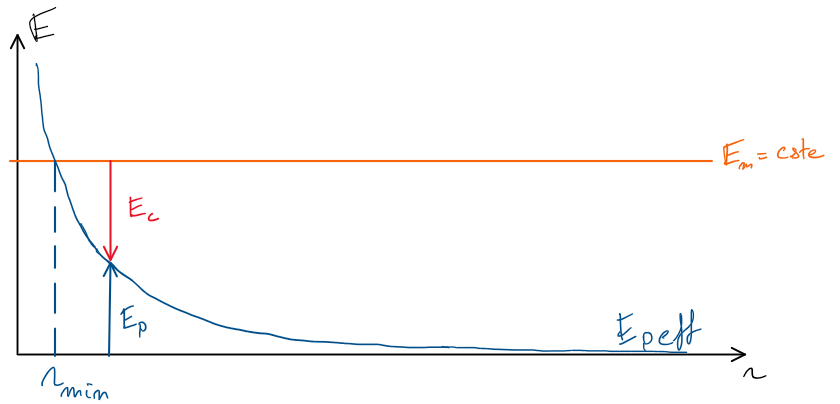
\includegraphics[width=0.8 \textwidth]{SCHEMA3-4.png}
    \caption{Représentation graphique du cas 1}
    \label{fig:SCHEMA3-4}
\end{figure}

Indépendamment des conditions initiales, on a un mouvement qui n'est pas borné : \(r \in \left[ r_{\min} ; \infty \right]\). On parle d'un état de diffusion. 
\newpage
\subsubsection{2eme cas : \(k<0\)}

\begin{figure}[!htb]
    \centering
    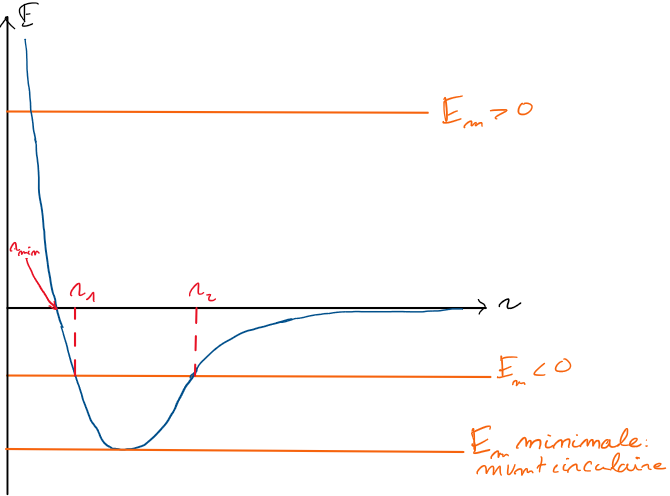
\includegraphics[width=0.7 \textwidth]{SCHEMA3-5.png}
    \caption{Représenation graphique du cas 2}
    \label{fig:SCHEMA3-5}
\end{figure}



\paragraph{Si \(E_{m} \geq 0\)}
Le mouvement est toujours non borné. \(r \in \left[ r_{\min} ; \infty \right]\), on retrouve l'état de diffusion.
\paragraph{Si \(E_{m} < 0 \) }
Si \(E_{m} <0 \), le mouvement est borné, \(r \in \left[ r_{1}; r_{2} \right]\), on est dans un état lié.
\begin{corollary}[Calcul de \(r_{1}\) et \(r_{2}\)  ]
    \begin{align*}
        E &= \frac{1}{2}m\dot{r}^{2} + \frac{k}{r} + \frac{ml^{2}}{2r^{2}} = \text{cste} \\
        \intertext{Or pour \(r = r_{1}\) ou \(r=r_{2}\), on a \(\dot{r}=0\)}
        E &= \frac{k}{r} + \frac{ml^{2}}{2r^{2}} \\
        2Er^{2}-2kr - ml^{2} &= 0 \\
        \implies \Delta &= 4k^{2}+8Eml^{2} \\
        \implies \left(r_{1}; r_{2}\right) &= \left( \frac{k - \sqrt{k^{2}+2Eml^{2}}}{2E} ; \frac{k+\sqrt{k^{2} + 2Eml^{2}}}{2E} \right)
    \end{align*}
\end{corollary}

\section{Mouvment dans un champ de force centrale attractive}
\subsection{Formule de Binet}

\begin{theorem}[Formule de Binet]
    On étudie un point matériel \(M\) de masse \(m\) dans un champ de force central. On a alors :
    \[
        \vv{a} = -l^{2}u^{2}\left( \frac{d^{2}u}{d \theta^{2}} + u \right) \vv{u}_{r}, u = \frac{1}{r}
    \]
\end{theorem}
\newpage
\begin{explanation}
    On rappelle que : 
    \[
        \begin{cases}
            \vv{OM} = r\vv{u}_{r} \\
            \vv{v} = \dot{r}\vv{u}_{r} + r\dot{\theta}\vv{u}_{\theta} \\
            \vv{a} = \left(\ddot{r}-r\dot{\theta}^{2}\right)\vv{u}_{r} + (r \ddot{\theta} + 2\dot{r}\dot{\theta})
        \end{cases}
    \]  
    Or on a \(r^{2}\dot{\theta} = l = \text{cste}\). 
    \begin{align*}
        \implies \frac{d}{dt}\left( r^{2} - \dot{\theta} \right) &= 0 \\
        \implies 2r\dot{r}\dot{\theta} +r^{2}\ddot{\theta} &= 0 \\
        \implies r\left( 2\dot{r}\dot{\theta} + r \ddot{\theta} \right) &= 0 \\
        \implies 2\dot{r}\dot{\theta} + r \ddot{\theta} &= 0 \\
        \implies \vv{a} = \left( \ddot{r} - r \dot{\theta}^{2} \right)\vv{u}_{r}
    \end{align*}
    On pose \(u = \frac{1}{r} \iff r = \frac{1}{u}\). On cherche à calculer \(\dot{r}\) et \(\ddot{r}\). \par
    Calcul de \(\dot{r}\) : 
    \begin{align*}
        \dot{r} &= \frac{d}{dt} \left( \frac{1}{u} \right) \\
        &= \frac{d \theta}{dt} \times \frac{d}{d \theta} \frac{1}{u}\\
        &= \dot{\theta}\left( -\frac{1}{u^{2}} \frac{du}{d \theta} \right) \\
        \intertext{Or \(r^{2}\dot{\theta} = l \implies \dot{\theta} = \frac{l}{r^{2}}  = lu^{2}\) }
        &= lu^{2}\left( -\frac{1}{u^{2}} \frac{d^{2}u}{d \theta} \right)\\
        &= -l \frac{du}{d \theta}
    \end{align*}
    Calcul de \(\ddot{r}\) : 
    \begin{align*}
        \ddot{r} &= \frac{d}{dt}\dot{r} \\
        &= \frac{d \theta}{dt} \frac{d}{d \theta}\left( -\frac{ldu}{d \theta} \right) \\
        &= lu^{2} -l \frac{d^{2}u}{d \theta^{2}}\\
        \ddot{r} &= -l^{2}u^{2} \frac{d^{2}u}{d \theta^{2}}
    \end{align*}
    D'où on a donc :
    \[
        \vv{a} = -l^{2}u^{2} \left[ \frac{d^{2}u}{d \theta^{2}} +u  \right] \vv{u}_{r}
    \] 
\end{explanation}

